\documentclass[12pt]{article}
\usepackage[utf8]{inputenc}
\usepackage[brazil]{babel}
\usepackage{amsmath, amssymb}
\usepackage{geometry}
\usepackage{graphicx}
\geometry{a4paper, margin=2cm}

% ------------------------------------------------------
%  PROVA 3 – Estruturas de Dados e Algoritmos (PCC104)
% ------------------------------------------------------

\title{PCC104 – Prova 3}
\author{Universidade Federal de Ouro Preto}
\date{}

\begin{document}

\maketitle

\noindent\textbf{Nome do(a) aluno(a):} \rule{11cm}{0.4pt}

\bigskip

\begin{enumerate}

  \item (\textbf{2~pt}) Apresente a análise de complexidade de \emph{pior caso}, em número de comparações, da sua implementação do algoritmo \textit{Selection Sort}. 
  \medskip
  
  \item (\textbf{2~pt}) Considere a sua implementação de \textit{heap}. Descreva o comportamento do programa quando o usuário tenta inserir uma chave que já está presente na estrutura. Justifique citando os trechos de código relevantes.
  \medskip

  \item (\textbf{2~pt}) Apresente a análise de complexidade do método \texttt{search} da sua Árvore Binária nos seguintes cenários:
  \begin{enumerate}
    \item árvore perfeitamente balanceada;
    \item árvore degenerada (todos os nós à direita ou à esquerda).
  \end{enumerate}
  \medskip

  \item (\textbf{2~pt}) Numere as células do labirinto abaixo seguindo a ordem em que são removidas da fronteira (\emph{frontier}) pela sua implementação do algoritmo de Busca em Largura (\emph{Breadth‑First Search}). Comece do vértice de origem, \textbf{s}. O objetivo é chegar até \textbf{g}. 
  \begin{figure}[h]
    \centering
    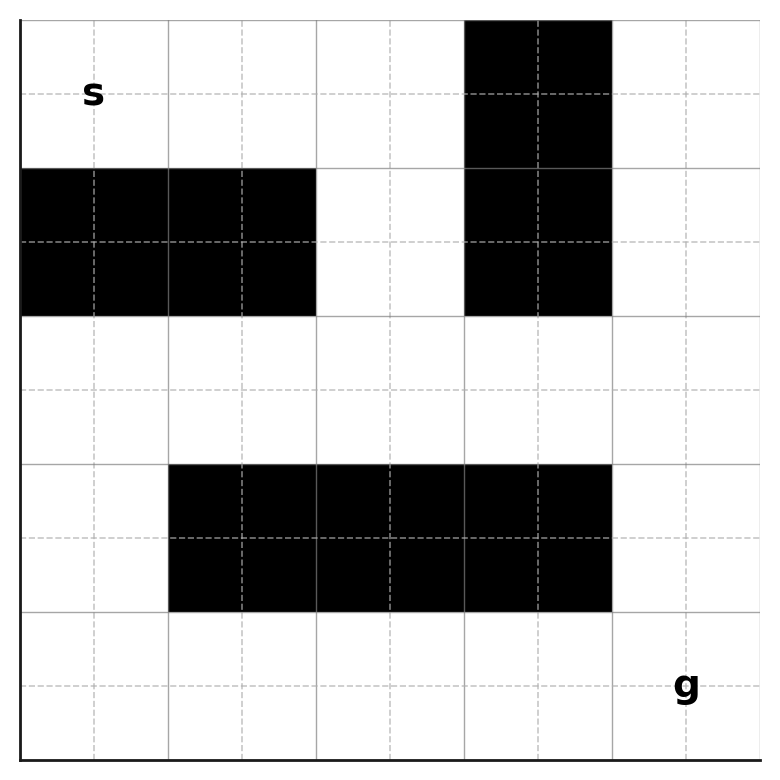
\includegraphics[width=.45\textwidth]{maze.png}
  \end{figure}
  \medskip

 \item (\textbf{2~pts}) Considere um conjunto de $n$ turmas, cada uma com um número de estudantes $s_i$, e um conjunto de $m$ salas, cada uma com capacidade $c_j$ ($1 \leq i \leq n$, $1 \leq j \leq m$). Deseja-se atribuir cada turma a exatamente uma sala de forma que $s_i \leq c_{\text{(sala atribuída)}}$. Caso não exista atribuição viável para todas as turmas, o algoritmo deve sinalizar falha. Escreva um algoritmo em \emph{pseudocódigo} utilizando \textbf{backtracking} que encontre uma alocação válida (ou indique que ela não existe). Você pode definir métodos auxiliares se achar necessário.

\end{enumerate}

\end{document}
